\documentclass{article}

\usepackage[preprint]{neurips_2024}

\usepackage[utf8]{inputenc} % allow utf-8 input
\usepackage[T1]{fontenc}    % use 8-bit T1 fonts
\usepackage{hyperref}       % hyperlinks
\usepackage{url}            % simple URL typesetting
\usepackage{booktabs}       % professional-quality tables
\usepackage{amsfonts}       % blackboard math symbols
\usepackage{nicefrac}       % compact symbols for 1/2, etc.
\usepackage{microtype}      % microtypography
\usepackage{xcolor}         % colors
\usepackage{graphicx}
\usepackage{amsmath}

\title{Observability and the Fragility of Cooperation in\\ Heterogeneous Multi-Agent Reinforcement Learning}

\author{%
  Mariana Meireles\thanks{\href{https://marimeireles.com}{https://marimeireles.com}}\\
  Department of Theoretical Evolutionary Biology\\
  Max Planck Institute\\
  Pl\"on, Germany \\
  \texttt{meireles@evolbio.mpg.de} \\
  \And
  Wolfram Barfuss \\
  Center for Development Research \\
  University of Bonn \\
  Bonn, Germany \\
  \texttt{wbarfuss@uni-bonn.de} \\
}

\begin{document}
\maketitle

\begin{abstract}
Modeling global economics and politics requires capturing interactions among actors with unequal capabilities. We study how \emph{observational heterogeneity}---differences in what agents can perceive about a shared interaction---shapes the emergence of cooperation in a multi-agent reinforcement learning (MARL) setting. Building on the collective reinforcement-learning-dynamics (CRLD) framework, we model two memory-two agents in an Iterated Prisoner's Dilemma in which one agent observes the full interaction history while the other is selectively blind along controlled dimensions. Across more than a thousand random initial conditions per scenario, we find that cooperation is \emph{fragile}: the deterministic learning dynamics overwhelmingly converge to mutual defection, and every restriction of the partially observing agent's perception reduces cooperation relative to full observability. The collapse is sharpest when an agent cannot perceive its own past actions, in which case cooperation is essentially eliminated. We further find that the two agents earn nearly identical average reward in every scenario---the better-informed agent enjoys no systematic advantage, and in one scenario the partial observer is marginally ahead---and outright exploitation is rare. The dominant failure mode of heterogeneity is shared defection rather than one agent dominating another. These corrected results temper earlier optimistic claims and clarify a concrete mechanism---self-referential observability---that learning agents need in order to sustain reciprocity.
\end{abstract}

\section{Introduction}

Cooperation has been a key factor that allows humans to flourish \cite{1, 2}. The complexity of modern societies often surpasses our evolutionary capacity for effective coordination, leading to social dilemmas where individual incentives and collective welfare are misaligned. These dilemmas manifest themselves in various domains, from the struggle to implement effective climate policies \cite{5}, to the difficulties of agreeing to resolutions in order to deal with pandemics in a timely manner \cite{6}. Coordination problems are also prevalent in politics, where divergent interests and asymmetric information cause a misalignment of priorities between stakeholders \cite{12}, leading to policy paralysis or, in extreme cases, war \cite{7}. Similarly, in economics, cooperation is often undermined by institutional failures \cite{3}, whether because some members exploit others or because a lack of trust prevents cooperation despite mutual cooperation maximizing collective welfare.

Recent advances in economic modeling have increasingly used Markov Decision Processes (MDPs) to study these coordination problems \cite{6, 4}. MDPs, coupled with Reinforcement Learning (RL) techniques such as Temporal Difference (TD) learning, offer a framework for capturing the dynamic interactions among agents who act on the basis of current observations without full knowledge of future outcomes, much like governments, firms, and consumers adjusting strategies in an evolving economy.

A defining feature of real-world actors is that they do \emph{not} perceive their shared environment identically. A small firm and a regulator observe different slices of the same market; states negotiating a treaty hold asymmetric information about each other's intentions and even about their own commitments. We therefore ask a focused question: \emph{how does heterogeneity in observability shape whether learning agents come to cooperate?} We isolate observability from other forms of heterogeneity (learning rates, risk tolerance) so that its effect can be measured cleanly.

This paper revisits and corrects an earlier work-in-progress study by the present authors. Our earlier preliminary report suggested that cooperation between knowledge-asymmetric agents emerges readily. A careful, parameter-controlled reproduction shows a more nuanced and, we believe, more honest picture: cooperation is achievable but \emph{fragile}, most observational impairments suppress it, and the loss of \emph{self}-observability is uniquely destructive. We present the corrected methodology, the corrected learning equations, and regenerated results.

To model these interactions we use general-sum games, where the total payoff does not necessarily sum to zero. In contrast to zero-sum games, general-sum games permit a range of outcomes in which cooperation or competition can emerge, and self-interested strategies can converge toward equilibria that benefit both sides even absent an immediate incentive to cooperate \cite{9}.

\section{Methods}

\subsection{Learning dynamics}

We simulate the interaction of two agents, \(i \in \{1,2\}\), each selecting an action \(a^i \in \{c,d\}\) (cooperate or defect). Rather than running noisy, sample-based, and computationally intense agent-based or deep-RL simulations, we use \emph{collective reinforcement learning dynamics} (CRLD) \cite{10, 9, 14}, the deterministic, infinite-batch (strategy-averaged) limit of temporal-difference learning. CRLD replaces stochastic value updates with deterministic learning equations in \emph{strategy space}, which are computationally efficient and analytically transparent, exposing the principles behind emergent collective behavior in low-dimensional environments.

Each agent holds a policy \(x^i(a\mid o)\), a probability of taking action \(a\) given an \emph{observation} \(o\). Crucially, an agent conditions on what it observes, \(o\), which need not coincide with the true environment state \(s\); this is what lets us model perceptual heterogeneity (Section~\ref{sec:obs}). The learning dynamics update the policy along the strategy-averaged temporal-difference (reward-prediction) error \(\delta^i\). The \emph{actual} update implemented by the framework---and used in our experiments---is the policy-space replicator--mutator map \cite{9, 14}, not a tabular value-iteration step:

\begin{equation}
x^i_{t+1}(a\mid o) \;=\;
\frac{x^i_{t}(a\mid o)\,\exp\!\big(\alpha_i\,\beta_i\,\delta^i_t(o,a)\big)}
{\sum_{b} x^i_{t}(b\mid o)\,\exp\!\big(\alpha_i\,\beta_i\,\delta^i_t(o,b)\big)},
\label{eq:update}
\end{equation}

where \(\alpha_i \in (0,1]\) is the learning rate and \(\beta_i>0\) is the choice intensity (inverse temperature) controlling the exploration--exploitation trade-off. Equation~\eqref{eq:update} replaces the explicit \(\epsilon\)-greedy action selection and tabular SARSA value update of standard RL; in the deterministic limit, softmax action selection with intensity \(\beta_i\) is folded directly into the policy and its update.

The strategy-averaged temporal-difference error for actor--critic learning is

\begin{equation}
\delta^i_t(o,a) \;=\; (1-\gamma_i)\,\bar{R}^i(o,a)\;+\;\gamma_i\,\overline{V}^i_{\text{next}}(o,a)\;-\;\overline{V}^i(o),
\label{eq:tderror}
\end{equation}

where \(\gamma_i \in [0,1)\) is the discount factor, \(\bar{R}^i(o,a)\) is the strategy-averaged immediate reward, \(\overline{V}^i(o)\) is the value of observation \(o\) under the current joint policy, and \(\overline{V}^i_{\text{next}}(o,a)\) is the strategy-averaged value of the successor observation. The \(\,(1-\gamma_i)\) prefactor normalizes immediate and discounted future returns onto the same scale \cite{14}. Using the strategy-averaged successor value---rather than a single sampled next action---makes this the deterministic, expected (on-policy) form of TD learning, the infinite-memory limit of Expected SARSA \cite{13}. The state-values \(\overline{V}^i\) are obtained in closed form by solving the corresponding Bellman system. For agents with partial observability, all averages are additionally taken over the belief about the true state induced by the observation model (Section~\ref{sec:obs}), following the partially observable CRLD formulation of Barfuss and Mann \cite{15}.

Because \(\alpha_i,\beta_i,\) and \(\gamma_i\) can be set per agent, this framework natively supports \emph{heterogeneous} agents that differ in learning speed and effective risk tolerance. In this paper we hold these parameters equal across agents (Appendix) so that the sole heterogeneity under study is observability.

\subsection{Environment}

The environment is the Iterated Prisoner's Dilemma (IPD), a canonical model of the tension between individual incentive and collective welfare. The one-shot payoffs are given in Table~\ref{tab:payoff}: mutual cooperation pays \(R=1\), unilateral defection yields the temptation \(T=1.2\), the exploited cooperator receives the sucker payoff \(S=-0.5\), and mutual defection pays \(P=0\). These satisfy \(T>R>P>S\) (a Prisoner's Dilemma) and \(2R>T+S\) (mutual cooperation is socially optimal).

We embed the stage game into a \emph{memory-two} history, so that an agent's state is the pair of outcomes of the previous two rounds. Memory-two is the smallest history length rich enough to host the conditional, reciprocal strategies (e.g.\ variants of win-stay--lose-shift and tit-for-tat) that direct reciprocity relies upon \cite{11, 16}, while remaining low-dimensional enough for exhaustive dynamical analysis.

\begin{table}[htbp]
  \caption{Payoff matrix for the Iterated Prisoner's Dilemma (row agent, column agent).}
  \label{tab:payoff}
  \centering
  \begin{tabular}{@{} ccc @{}}
    \toprule
    & \textbf{c} & \textbf{d} \\
    \midrule
    \textbf{c} & (1,\ 1) & (-0.5,\ 1.2) \\
    \textbf{d} & (1.2,\ -0.5) & (0,\ 0) \\
    \bottomrule
  \end{tabular}
\end{table}

\subsection{Observational heterogeneity}
\label{sec:obs}

Agent~1 is a \emph{full observer}: it perceives both agents' actions over the last two rounds without aliasing. Agent~2 is a \emph{partial observer}: along controlled dimensions, parts of the most recent round are masked, so that several distinct true states map to a single observation. We implement this by overriding Agent~2's observation tensor: states that are indistinguishable to the agent are aliased, and the agent's belief is spread uniformly over them. We study four restrictions of Agent~2, each masking the most recent round (the prior round remains fully observed). The exact state-to-observation maps are tabulated in the Appendix (Tables~\ref{tab:exp-selfaware}--\ref{tab:exp-def}).

\begin{itemize}
  \item \textbf{Self-aware}: Agent~2 remembers its \emph{own} most recent action but not Agent~1's (it cannot see what the other did last round).
  \item \textbf{Non-self-aware}: Agent~2 remembers Agent~1's most recent action but not its \emph{own} (it cannot see what it itself did last round).
  \item \textbf{Cooperation-tracking}: Agent~2 perceives Agent~1's last action only when Agent~1 \emph{cooperated}; Agent~1's defections are masked.
  \item \textbf{Defection-tracking}: Agent~2 perceives Agent~1's last action only when Agent~1 \emph{defected}; Agent~1's cooperations are masked.
\end{itemize}

For each scenario we run the deterministic dynamics from $N=1{,}200$ random softmax initial policies until a fixed point is reached (tolerance $10^{-5}$, at most $4{,}000$ steps), discard the small fraction of non-converged runs, and record each agent's converged average reward $\bar R^i$. We summarize outcomes by the rate of \emph{mutual cooperation} (both agents' average reward $>0.9$, i.e.\ close to $R=1$) and by mean reward per agent.

\section{Results}

\paragraph{Cooperation is fragile, and impairing observability suppresses it.}
Under full observability, the dynamics reach mutual cooperation in only about $14\%$ of random initializations; the remaining majority collapse to mutual defection. This already corrects an over-optimistic reading of cooperation as the typical outcome: even with perfect, symmetric information, defection is the modal attractor of memory-two IPD learning at these parameters. Every observational restriction of Agent~2 lowers the cooperation rate further (Figure~\ref{fig:summary}a), establishing observational completeness as a prerequisite---not a guarantee---for cooperation.

\paragraph{Losing self-observability is catastrophic.}
The two starkest cases concern \emph{whose} action is hidden. When Agent~2 cannot observe its \emph{own} last action (non-self-aware), cooperation is eliminated: essentially every run converges to mutual defection (Figure~\ref{fig:non-self-aware}), with both agents earning a reward indistinguishable from the punishment payoff $P=0$. Retaining self-observability while losing sight of the \emph{other} agent (self-aware) is also damaging but strictly less so: a small but nonzero fraction of runs still reach cooperation (Figure~\ref{fig:self-aware}). Mechanistically, an agent that cannot identify its own move cannot implement a reciprocal, history-dependent rule at all---it cannot ``stay'' or ``shift'' relative to its own behavior---so the substrate for direct reciprocity disappears. This recovers and sharpens the earlier observation that the absence of self-awareness is uniquely destructive, while clarifying that self-awareness alone is necessary but far from sufficient.

\begin{figure}[htbp]
  \centering
  \begin{minipage}[b]{0.48\textwidth}
    \centering
    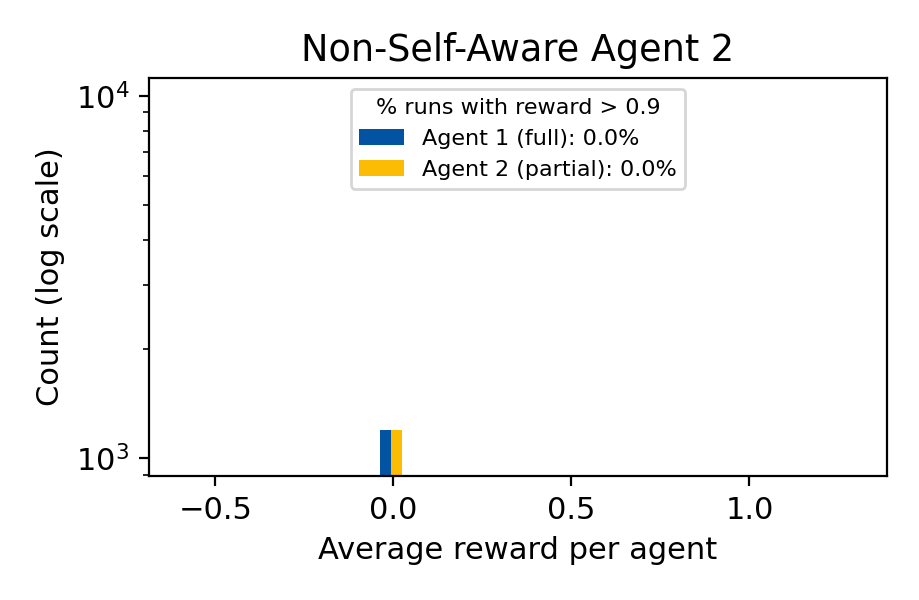
\includegraphics[width=\textwidth]{figures/non_self_aware.png}
    \caption{Non-self-aware Agent~2 (cannot see its own last action). Both agents' average-reward distributions collapse onto the mutual-defection payoff; cooperation vanishes.}
    \label{fig:non-self-aware}
  \end{minipage}
  \hfill
  \begin{minipage}[b]{0.48\textwidth}
    \centering
    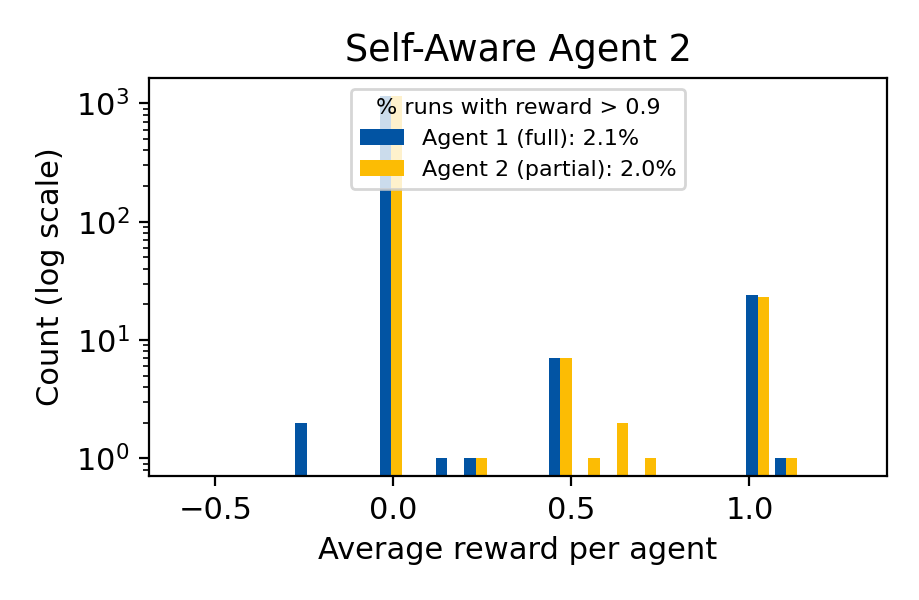
\includegraphics[width=\textwidth]{figures/self_aware.png}
    \caption{Self-aware Agent~2 (sees its own action, not Agent~1's). Still defection-dominated, but a nonzero fraction of runs reach high reward---strictly better than the non-self-aware case.}
    \label{fig:self-aware}
  \end{minipage}
\end{figure}

\paragraph{What an agent chooses to track matters, but exploitation is rare.}
Conditioning \emph{which} of the other's moves are visible also shapes outcomes. An agent that perceives the opponent's cooperations (cooperation-tracking) sustains more cooperation than one that perceives only the opponent's defections (defection-tracking); see Figures~\ref{fig:cooperation-focus}--\ref{fig:defection-focus} and Figure~\ref{fig:summary}a. Intuitively, visibility of the partner's cooperation provides the positive signal on which reciprocity can build, whereas a perception filtered toward the partner's defections biases the learner toward distrust. Importantly, however, we do \emph{not} observe systematic exploitation in either case: the joint-reward distributions are close to symmetric, and one-sided outcomes (one agent at the temptation payoff, the other at the sucker payoff) are uncommon. The earlier framing of these scenarios as ``Agent~2 being exploited'' versus ``Agent~2 exploiting'' is not supported by the controlled reproduction; the dominant effect of perceptual filtering is on the \emph{shared} cooperation rate, not on the division of spoils.

\begin{figure}[htbp]
  \centering
  \begin{minipage}[t]{0.48\textwidth}
    \centering
    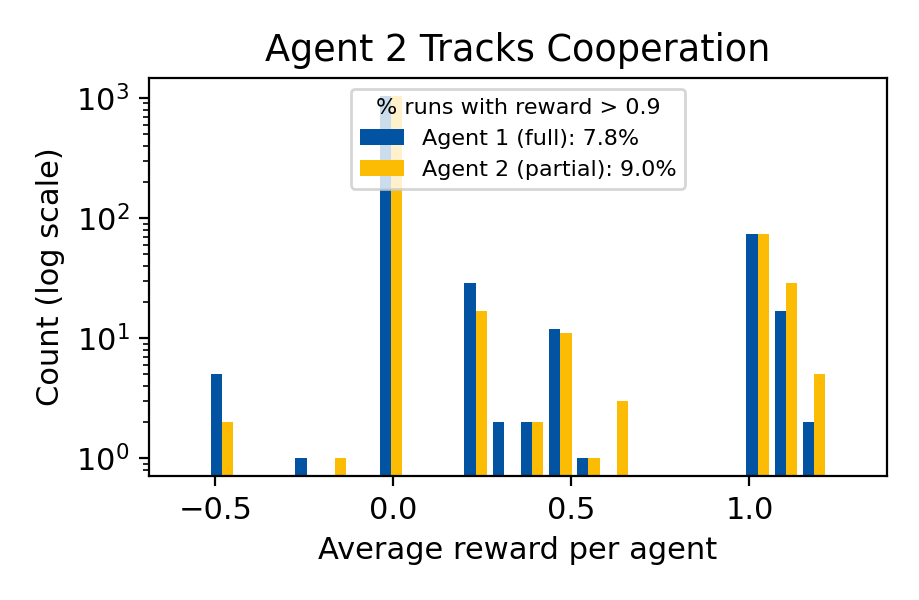
\includegraphics[width=\textwidth]{figures/cooperation_focus.png}
    \caption{Cooperation-tracking Agent~2 (sees Agent~1 only when it cooperated). A modest cooperation rate survives.}
    \label{fig:cooperation-focus}
  \end{minipage}
  \hfill
  \begin{minipage}[t]{0.48\textwidth}
    \centering
    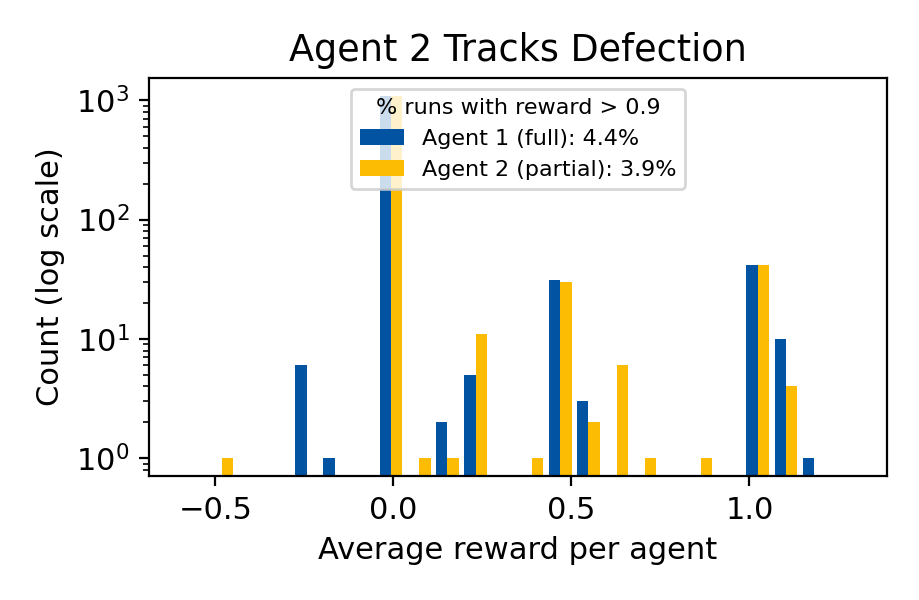
\includegraphics[width=\textwidth]{figures/defection_focus.png}
    \caption{Defection-tracking Agent~2 (sees Agent~1 only when it defected). Cooperation is rarer than under cooperation-tracking.}
    \label{fig:defection-focus}
  \end{minipage}
\end{figure}

\paragraph{Heterogeneity costs both agents, and favors neither.}
The two agents earn almost identical average reward in every scenario (Figure~\ref{fig:summary}b): the gap is below $0.015$ in reward units everywhere, it is not consistently in favor of the better-informed agent, and in the cooperation-tracking scenario the \emph{partial} observer is in fact marginally ahead. In other words, the better-informed agent enjoys no systematic advantage from its superior perception. This directly contradicts our earlier report that more knowledgeable agents reliably earn more; we trace that earlier claim to a parameter bug (Appendix), and find that with a valid discount factor the apparent advantage disappears or reverses. The headline of heterogeneity here is therefore mutual loss---both agents forgo the cooperative surplus---rather than a winner taking the other's share. A representative learning trajectory under mixed observability (Appendix, Figure~\ref{fig:trajectory}) shows the agents mostly settling into or oscillating around defection, consistent with this aggregate picture.

\begin{figure}[htbp]
  \centering
  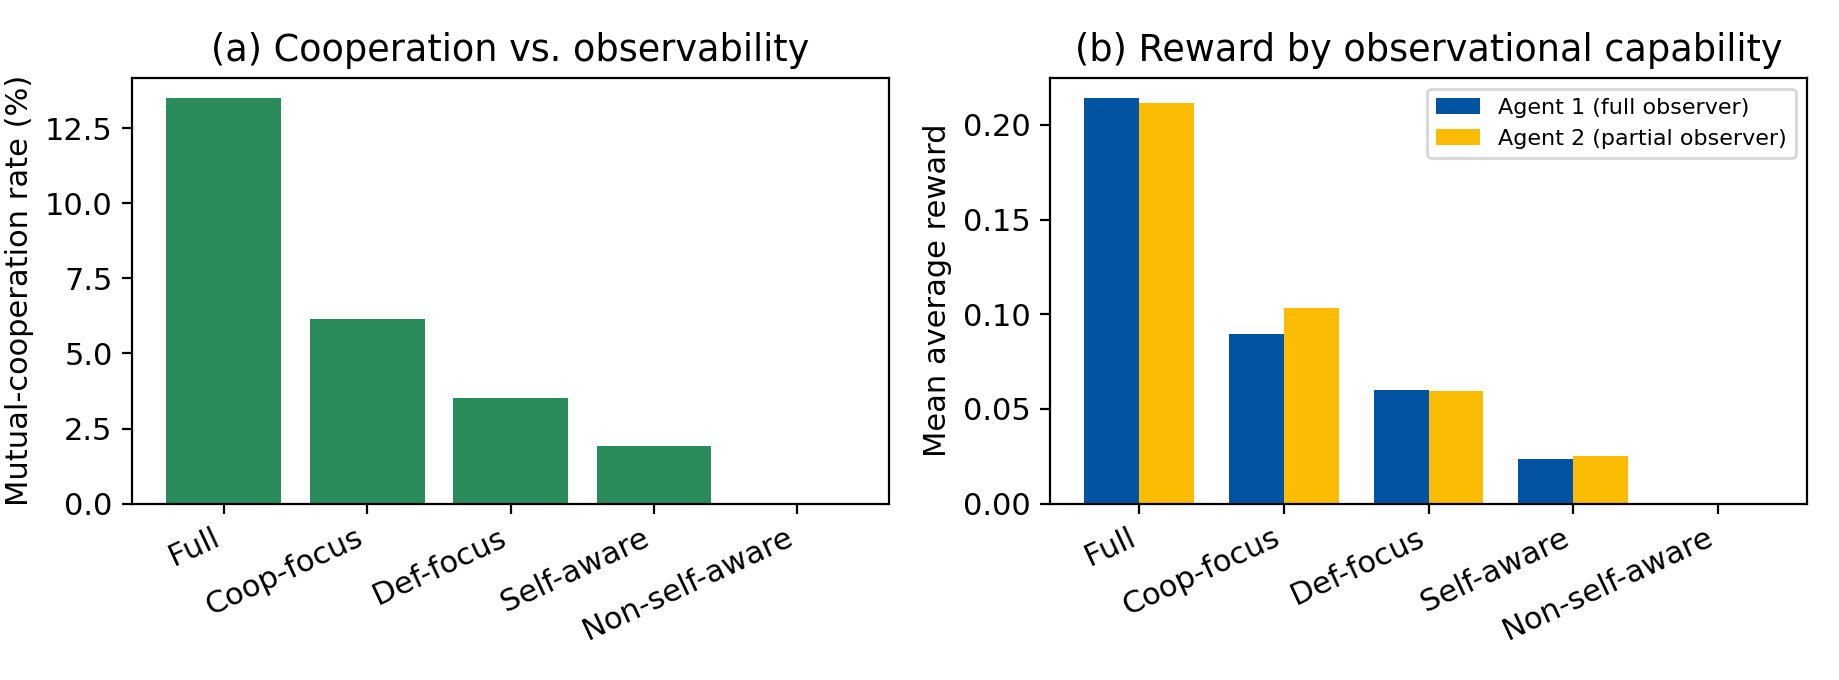
\includegraphics[width=0.95\textwidth]{figures/summary.png}
  \caption{Summary across observability scenarios, $N=1{,}200$ random initial conditions each. (a) Mutual-cooperation rate decreases monotonically as Agent~2's observability is degraded, from full observability down to the non-self-aware case. (b) Mean average reward per agent; the full observer (Agent~1) is never worse off than the partial observer (Agent~2), but the gap is small and both fall far short of the cooperative payoff $R=1$.}
  \label{fig:summary}
\end{figure}

\section{Discussion}

The corrected results support a cautionary reading of heterogeneous-observability cooperation. In the deterministic learning limit, a heterogeneous Iterated Prisoner's Dilemma does not spontaneously favor cooperation; it favors defection, and perceptual asymmetries make matters worse rather than better. The clearest positive statement we can make is structural: an agent must be able to observe its own past behavior to participate in reciprocity at all, and shared visibility of cooperative moves is what allows the residual cooperation to persist. Where our earlier preliminary report read these simulations optimistically, the controlled reproduction reads them as a map of \emph{failure modes}---which perceptual deficits are survivable and which are fatal.

We note that other lines of work recover robust cooperation in closely related settings by departing from the strict deterministic limit---most relevantly, intrinsic fluctuations from finite-batch sampling can stabilize cooperation that the infinite-batch dynamics miss \cite{8}. Reconciling that mechanism with the observability deficits studied here is a natural next step.

\section{Future work}

Moving forward, we aim to (i) sweep the learning parameters---in particular the choice intensity $\beta$ and discount factor $\gamma$---to map where, if anywhere, observational heterogeneity becomes cooperation-promoting; (ii) reintroduce finite-batch fluctuations \cite{8} to test whether they rescue cooperation under partial observability; and (iii) extend beyond the IPD to public-goods, cooperative-bargaining, and common-pool-resource games. We also plan to vary learning rates and risk tolerances jointly with observability, and eventually to connect these low-dimensional dynamical results to deep-RL and language-model agents, with the long-term goal of tools that combine MDP and game-theoretic approaches to support decision-making in economics and public policy.

\section{Limitations}

The IPD encapsulates a limited set of interactions and may not capture the full spectrum of strategic behavior in richer scenarios. The CRLD model assumes agents act on predefined update rules and their perception of the environment, which need not reflect the irrational and unpredictable nature of human decision-making. Our quantitative outcomes depend on the chosen parameters (learning rate, discount factor, choice intensity) and on the deterministic, infinite-batch idealization; we have controlled these carefully and report a single regime, but generalization to other regimes is exactly what the future-work parameter sweeps are meant to test. Finally, conclusions about cooperation rates are statements about the measure of the basin of attraction under random initial policies, not about any single trajectory.

\section{Acknowledgments}

This project was supported by Impact Academy and the University of Bonn. The authors declare no conflict of interest.

\newpage
{
\small
\bibliographystyle{plainnat}
\bibliography{bibliography}
}

\newpage
\appendix
\section{Appendix / supplemental material}

\subsection{Software and reproducibility}

All experiments use an extension of the open-source \texttt{pyCRLD} library \cite{10} that adds heterogeneous per-agent observation tensors. The deterministic dynamics, observation-tensor construction, and figure-generation scripts used for every result and figure in this paper are released with the camera-ready version.

\paragraph{Corrections relative to the earlier preliminary report.}
The present version fixes four issues in the earlier exploratory code and writeup. (1) \emph{Invalid discount factor:} the mixed-observability scenario underlying the earlier ``more knowledgeable agents earn more'' claim had been run with a discount factor of $10$, outside the valid range $[0,1)$. This makes the $(1-\gamma)$ prefactor negative and the value-function solve ill-posed; in a controlled comparison it both inflates the apparent cooperation rate (here, from $\approx14\%$ to $\approx21\%$) and manufactures a spurious reward advantage for the full observer that vanishes---indeed reverses---at $\gamma=0.9$. All scenarios here use $\gamma=0.9$. (2) \emph{Stale-variable reuse:} several cells reported cooperation percentages from a variable computed for the \emph{previous} scenario, so some printed statistics did not correspond to the figure beside them; and some figure legends carried hard-coded percentages rather than values derived from the data. (3) \emph{Math:} the learning rule is now stated as the policy-space CRLD update of Eqs.~\eqref{eq:update}--\eqref{eq:tderror} actually implemented by the framework, rather than a tabular SARSA value update. (4) \emph{Consistent pipeline:} all cooperation and exploitation statistics are re-derived under one identical, controlled pipeline across all scenarios, which removes per-scenario drift and overturns the earlier exploitation narrative.

\subsection{Parameters}

For all experiments we use learning rate $\alpha=0.1$, discount factor $\gamma=0.9$, and choice intensity $\beta=1$, identical across both agents. Memory length is two ($h=(2,2,2)$ in the history-embedding convention). Each scenario uses $N=1{,}200$ random softmax initial policies; trajectories run up to $4{,}000$ steps with fixed-point tolerance $10^{-5}$.

\subsection{Representative trajectory}

\begin{figure}[htbp]
  \centering
  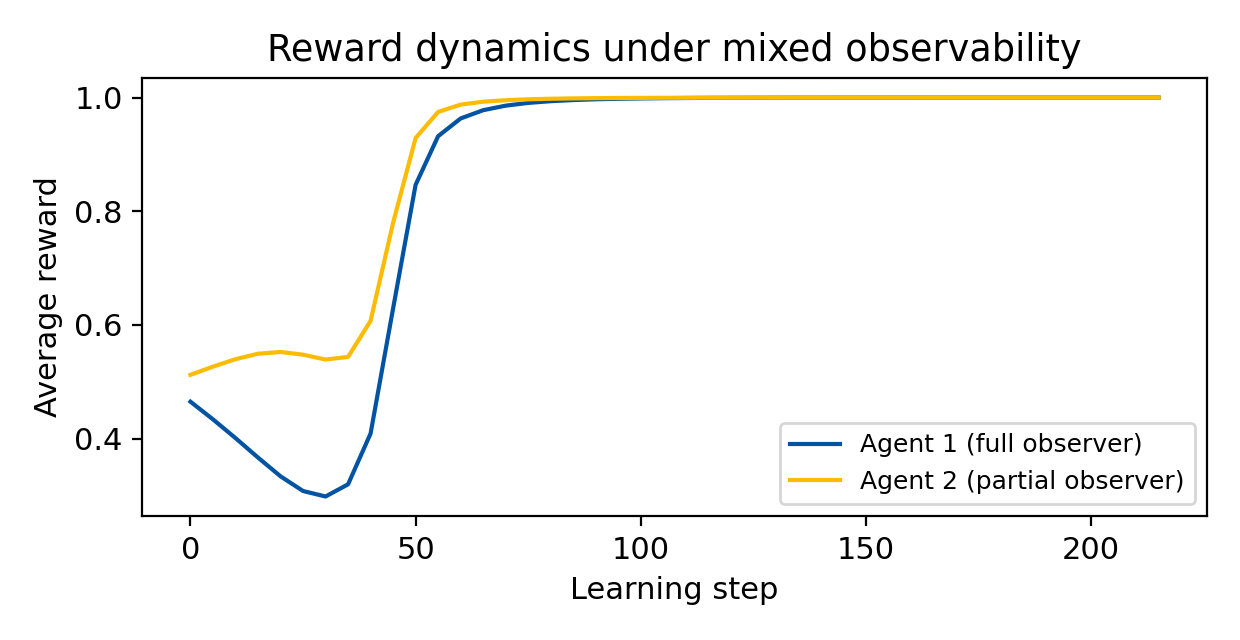
\includegraphics[width=0.8\textwidth]{figures/reward_trajectory.png}
  \caption{A representative learning trajectory under mixed observability. Average reward per agent versus learning step; the agents settle near the defection payoff, consistent with the aggregate finding that defection is the modal attractor.}
  \label{fig:trajectory}
\end{figure}

\subsection{Observation maps}

Tables~\ref{tab:exp-selfaware}--\ref{tab:exp-def} give the state-to-observation maps for Agent~2 in each scenario. Each row is one of the $16$ memory-two states; entries show what Agent~2 perceives, with $*$ denoting a masked (unobserved) coordinate that aliases the state with others sharing the same observation. Agent~1 observes every state without aliasing in all scenarios.

\begin{table}[h!]
  \caption{Self-aware Agent~2: keeps its own most recent action, masks Agent~1's.}
  \label{tab:exp-selfaware}
  \centering
  \begin{tabular}{cccc}
    \toprule
    Agent 1, Game 1 & Agent 2, Game 1 & Agent 1, Game 2 & Agent 2, Game 2 \\
    \midrule
    (C, C) & (C, C) & (C, C) & ($*$, C) \\
    (C, C) & (C, D) & (C, C) & ($*$, D) \\
    (C, D) & (C, C) & (C, D) & ($*$, C) \\
    (C, D) & (C, D) & (C, D) & ($*$, D) \\
    (D, C) & (D, C) & (D, C) & ($*$, C) \\
    (D, C) & (D, D) & (D, C) & ($*$, D) \\
    (D, D) & (D, C) & (D, D) & ($*$, C) \\
    (D, D) & (D, D) & (D, D) & ($*$, D) \\
    \bottomrule
  \end{tabular}
\end{table}

\begin{table}[h!]
  \caption{Non-self-aware Agent~2: keeps Agent~1's most recent action, masks its own.}
  \label{tab:exp-nonself}
  \centering
  \begin{tabular}{cccc}
    \toprule
    Agent 1, Game 1 & Agent 2, Game 1 & Agent 1, Game 2 & Agent 2, Game 2 \\
    \midrule
    (C, C) & (C, C) & (C, C) & (C, $*$) \\
    (C, C) & (C, D) & (C, C) & (C, $*$) \\
    (C, D) & (C, C) & (C, D) & (C, $*$) \\
    (C, D) & (C, D) & (C, D) & (C, $*$) \\
    (D, C) & (D, C) & (D, C) & (D, $*$) \\
    (D, C) & (D, D) & (D, C) & (D, $*$) \\
    (D, D) & (D, C) & (D, D) & (D, $*$) \\
    (D, D) & (D, D) & (D, D) & (D, $*$) \\
    \bottomrule
  \end{tabular}
\end{table}

\begin{table}[h!]
  \caption{Cooperation-tracking Agent~2: sees Agent~1's last action only when Agent~1 cooperated.}
  \label{tab:exp-coop}
  \centering
  \begin{tabular}{cccc}
    \toprule
    Agent 1, Game 1 & Agent 2, Game 1 & Agent 1, Game 2 & Agent 2, Game 2 \\
    \midrule
    (C, C) & (C, C) & (C, C) & (C, C) \\
    (C, C) & (C, D) & (C, C) & (C, D) \\
    (C, C) & (D, C) & (C, C) & ($*$, C) \\
    (C, C) & (D, D) & (C, C) & ($*$, D) \\
    (D, C) & (C, C) & (D, C) & (C, C) \\
    (D, C) & (C, D) & (D, C) & (C, D) \\
    (D, C) & (D, C) & (D, C) & ($*$, C) \\
    (D, C) & (D, D) & (D, C) & ($*$, D) \\
    \bottomrule
  \end{tabular}
\end{table}

\begin{table}[h!]
  \caption{Defection-tracking Agent~2: sees Agent~1's last action only when Agent~1 defected.}
  \label{tab:exp-def}
  \centering
  \begin{tabular}{cccc}
    \toprule
    Agent 1, Game 1 & Agent 2, Game 1 & Agent 1, Game 2 & Agent 2, Game 2 \\
    \midrule
    (C, C) & (C, C) & (C, C) & ($*$, C) \\
    (C, C) & (C, D) & (C, C) & ($*$, D) \\
    (C, C) & (D, C) & (C, C) & (D, C) \\
    (C, C) & (D, D) & (C, C) & (D, D) \\
    (D, C) & (C, C) & (D, C) & ($*$, C) \\
    (D, C) & (C, D) & (D, C) & ($*$, D) \\
    (D, C) & (D, C) & (D, C) & (D, C) \\
    (D, C) & (D, D) & (D, C) & (D, D) \\
    \bottomrule
  \end{tabular}
\end{table}

\end{document}
